\section{Data Types} 
\label{datatypes}

\subsection{Base data types}
\label{base-types}

\subsubsection{text}
\label{text}

\begin{figure}[h]
	\caption{Text example}
	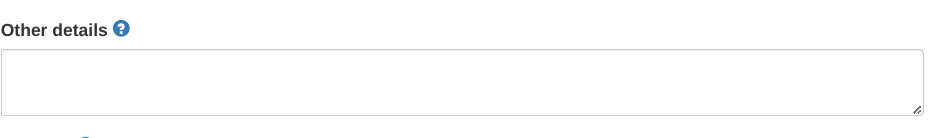
\includegraphics[width=10cm]{Textarea.png}
	\centering
\end{figure}

\subsubsection{string}
\label{string}

Simplest control type: a small rectangle accepting generic text.

\subsubsection{URN}
\label{URN}

Calculated by the server if \textbf{isFixed="true"}.
Server will generate a valid and unique URN for you.

\subsubsection{URI}
\label{URI}

Accepts a string and verifies it's an URI.

\subsubsection{URL}
\label{URL}
Accepts a string and verifies it's an URL.

\subsubsection{int}
\label{int}
Accepts a string and verifies it's an only contains numeric digits.

\subsubsection{float}
\label{real}

Accepts a string and verifies it's an only contains numeric digits or the decimal separator (i.e. a dot).

\begin{mdframed}
	With attribute \textbf{show="sliderfloat"}
	
	Shows a slider with a minimum and a maximum value and the position generates a value for this control.
	
	\begin{lstlisting}[language=xml]
		<item hasDatatype="float" show="sliderfloat" hasIndex="4" xml:id="slider2" isFixed="false" min="0.0" max="100.00" step="0.5">
		<label xml:lang="en">Slider Float 2</label>
		<label xml:lang="it">Slider Float 2</label>
		<defaultValue>49</defaultValue>
		<hasValue>70</hasValue>
		<hasPath>slider</hasPath>
		</item>
	\end{lstlisting}
	
	
	{\centering
		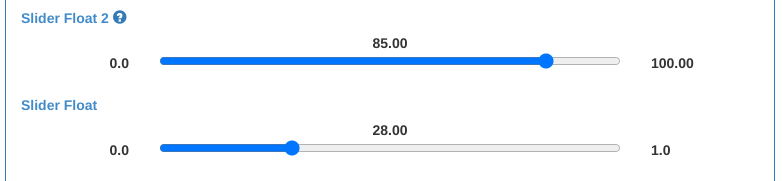
\includegraphics[width=10cm]{FloatSlider.png}
		\captionof{figure}{Example of floating-point control with sliderfloat}
		\par
	}
	
	
\end{mdframed}


Shows a slider with a minimum and a maximum value and the position generates a value for this control.

\begin{lstlisting}[language=xml]
	<item hasDatatype="float" show="sliderfloat" hasIndex="4" xml:id="slider2" isFixed="false" min="0.0" max="100.00" step="0.5">
	<label xml:lang="en">Slider Float 2</label>
	<label xml:lang="it">Slider Float 2</label>
	<defaultValue>49</defaultValue>
	<hasValue>70</hasValue>
	<hasPath>slider</hasPath>
	</item>
\end{lstlisting}


\subsubsection{real}
\label{double}

Same as \textit{float}.

\subsubsection{double}
\label{double}

Same as \textit{float}.


\subsubsection{codelist}
\label{codelist}

\begin{lstlisting}[language=xml]
	<item hasIndex="1" xml:id="ling_md_1" isLanguageNeutral="true" isFixed="false" hasDatatype="codelist" datasource="languages" show="combobox">
	<hasPath>/gmd:MD_Metadata/gmd:language/gmd:LanguageCode</hasPath>
	</item>
\end{lstlisting}
\begin{figure}[h]
	\caption{Codelist example with \textit{show="combobox"}}
	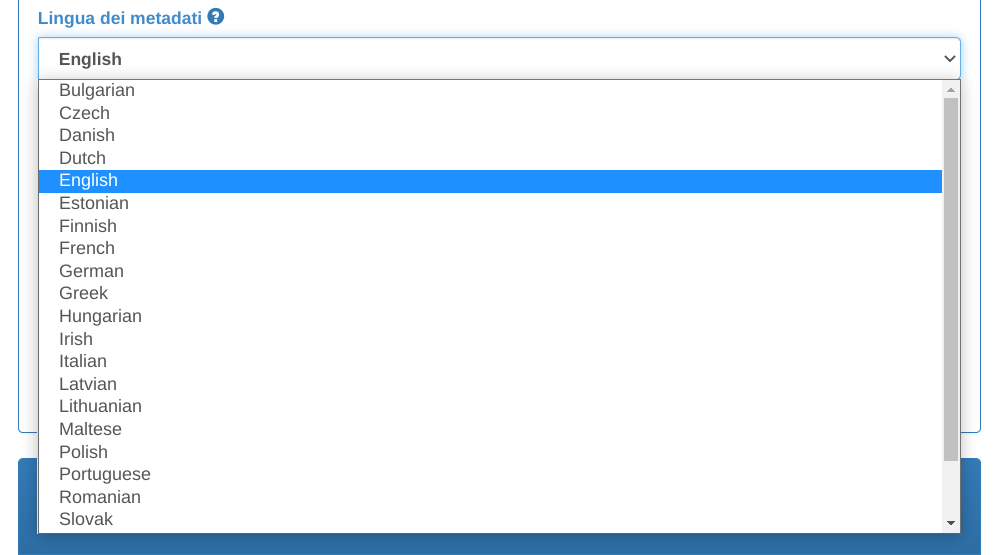
\includegraphics[width=10cm]{Codelist.png}
	\centering
\end{figure}

\subsubsection{autoCompletion}
\label{autoCompletion}

Similar to a \textit{codelist}, but preferrable with datasources containing many rows.

A textbox querying the datasource associated to the control for matching values.
Starts querying when at least 3 characters are entered.

\begin{lstlisting}[language=xml]
	<item hasIndex="1" xml:id="md_resp_1" outIndex="2" isFixed="false" hasDatatype="autoCompletion" datasource="person">
	<label xml:lang="en">Email</label>
	<label xml:lang="it">Email</label>
	<hasPath>/gmd:MD_Metadata/gmd:contact/gmd:CI_ResponsibleParty/gmd:contactInfo/gmd:CI_Contact/gmd:address/gmd:CI_Address/gmd:electronicMailAddress/gco:CharacterString</hasPath>
	</item>
\end{lstlisting}
\begin{figure}[h]
	\caption{AutoCompletion example}
	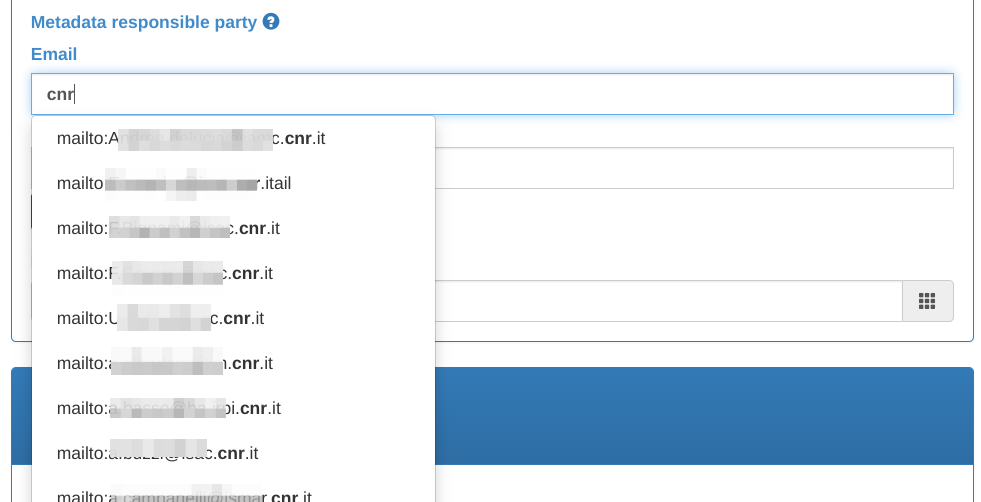
\includegraphics[width=10cm]{Autocompletion.png}
	\centering
\end{figure}


\subsubsection{boolean}
\label{boolean}

Shows a check-box, thus allowing only values \textbf{true} or \textbf{false}.


\subsection{Special case data types}
\subsubsection{label}
\label{label}

Shows read-only text.

\subsubsection{image}
\label{image}

Given an URL pointing to a valid image in the value, it shows the image.

\subsubsection{qrcode}
\label{qrcode}

Shows whatever the value is as a QR code.


\subsubsection{select}
\label{select}

The select datatype signifies that the item's value is based on some selection occurring in another item called a \textit{trigger item}.

It must be based on a data source of type \textbf{singleton} (see \ref{singleton}).

Sometimes the trigger item can be based on the same data source as its connected \textit{select} items, but it can be based on its own data source.

Each \textit{select} item must declare the field it represents in the datasouce.

\begin{lstlisting}[language=xml]
	<item hasIndex="2" xml:id="resp_2" outIndex="1" field="inst" isFixed="false" hasDatatype="select" datasource="personS_2">
	<label xml:lang="en">Institute</label>
	<label xml:lang="it">Ente</label>
	<hasPath>/gmd:MD_Metadata/gmd:identificationInfo/gmd:MD_DataIdentification/gmd:citation/gmd:CI_Citation/gmd:citedResponsibleParty/gmd:CI_ResponsibleParty/gmd:organisationName/gco:CharacterString</hasPath>
	</item>
\end{lstlisting}

\subsubsection{copy}
\label{copy}

\begin{figure}[h]
	\caption{String example, in this case it is part of a \textit{isMultiple="true"} element, as you can tell from the "+" button underneath it}
	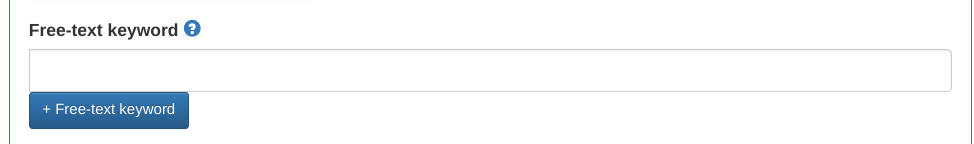
\includegraphics[width=10cm]{String.png}
	\centering
\end{figure}


% \subsubsection{dependent}
% \label{dependent}

\subsubsection{function}
\label{function}

Special data type.
Its value is calculated by the server by using its template \textit{hasValue} as an XPath run \textbf{against the parts of document that have already been generated}.

\subsubsection{ref}
\label{ref}

Special data type.
In the generated metadata document, it copies the Xpath specified in the \textit{hasValue} attribute to the Xpath specified by the \textit{hasPath} attribute.

\begin{lstlisting}[language=xml]
	<item hasDatatype="ref" hasIndex="7" xml:id="title_7" isFixed="true">
	<hasPath>dct:description/@xml:lang</hasPath>
	<hasValue>/rdf:RDF/dcatapit:Dataset/dct:title/@xml:lang</hasValue>
	</item>
\end{lstlisting}

In the example above, once the XML document is fully written, the \textbf{xml:lang} attribute of \textbf{dct:description} is set to equal the same attribute in \textbf{/rdf:RDF/dcatapit:Dataset/dct:title}.

\subsubsection{autonumber}
\label{autonumber}

Represents a value that's incremented every time it is encountered within the containing element.

Value is assigned by EDI Server.

\subsubsection{hidden}
\label{hidden}

Hidden item: it is \textit{fixed} by default (i.e. read-only).

\subsubsection{date}
\label{date}

Requests a date from the user, via a small calendar.

Requires a \textit{defaultValue}, which can be the macro \textit{\$TODAY\$}.

\begin{lstlisting}[language=xml]
	
	<item hasDatatype="date" hasIndex="7" xml:id="test_7" isFixed="false">
	<label xml:lang="en">Issues date</label>
	<label xml:lang="it">Data di rilascio</label>
	<help xml:lang="en">Help</help>
	<help xml:lang="it">Help</help>
	<hasValue>dct:issued</hasValue>
	<defaultValue>$TODAY$</defaultValue>
	</item>
	
\end{lstlisting}

\begin{figure}[h]
	\caption{Date example}
	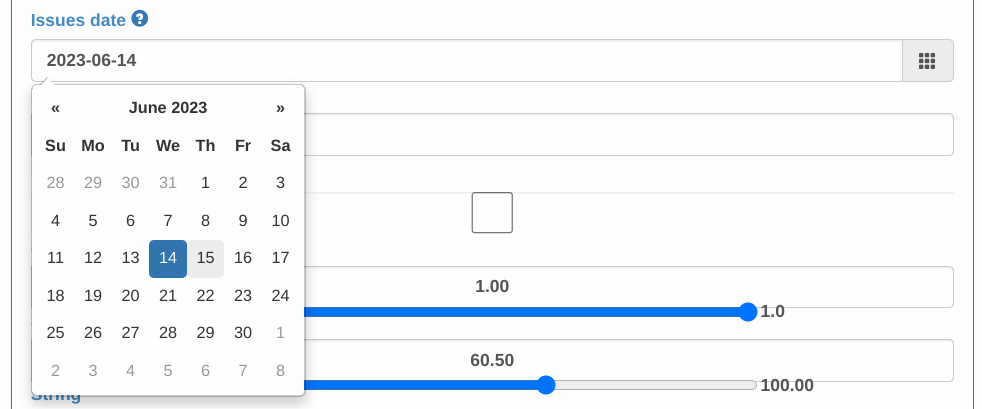
\includegraphics[width=10cm]{Date.png}
	\centering
\end{figure}


\subsubsection{dateRange}
\label{dateRange}

Same as \textit{date}, except that it requests a start and an end date.

\begin{lstlisting}[language=xml]
	
	<item hasIndex="8" xml:id="est_temp_8" isFixed="false" hasDatatype="dateRange">
	<label xml:lang="en">Start date</label>
	<label xml:lang="it">Data inizio</label>
	<start>
	<label xml:lang="en">Start date</label>
	<label xml:lang="it">Data inizio</label>
	<hasPath>/gmd:MD_Metadata/gmd:identificationInfo/gmd:MD_DataIdentification/gmd:extent/gmd:EX_Extent/gmd:temporalElement/gmd:EX_TemporalExtent/gmd:extent/gml:TimePeriod/gml:beginPosition</hasPath>
	</start>
	<end>
	<label xml:lang="en">End date</label>
	<label xml:lang="it">Data fine</label>
	<hasPath>/gmd:MD_Metadata/gmd:identificationInfo/gmd:MD_DataIdentification/gmd:extent/gmd:EX_Extent/gmd:temporalElement/gmd:EX_TemporalExtent/gmd:extent/gml:TimePeriod/gml:endPosition</hasPath>
	</end>
	</item>
	
\end{lstlisting}



\subsubsection{boundingBox}
\label{boundingBox}

Requests a geographic bounding box from the user.
It can be specified either by inputting the coordinates in 4 text boxes, or by drawing a rectangle on a map.

\begin{lstlisting}[language=xml]
	
	<item hasIndex="1" xml:id="loc_geo_1" isFixed="false" hasDatatype="boundingBox">
	<westLongitude outIndex="1" queryStringParameter="westlon">
	<label xml:lang="en">W longitude</label>
	<label xml:lang="it">Longitudine O</label>
	<hasPath>/gmd:MD_Metadata/gmd:identificationInfo/gmd:MD_DataIdentification/gmd:extent/gmd:EX_Extent/gmd:geographicElement/gmd:EX_GeographicBoundingBox/gmd:westBoundLongitude/gco:Decimal</hasPath>
	</westLongitude>
	<eastLongitude outIndex="2" queryStringParameter="eastlon">
	<label xml:lang="en">E longitude</label>
	<label xml:lang="it">Longitudine E</label>
	<hasPath>/gmd:MD_Metadata/gmd:identificationInfo/gmd:MD_DataIdentification/gmd:extent/gmd:EX_Extent/gmd:geographicElement/gmd:EX_GeographicBoundingBox/gmd:eastBoundLongitude/gco:Decimal</hasPath>
	</eastLongitude>
	<northLatitude outIndex="4" queryStringParameter="northlat">
	<label xml:lang="en">N latitude</label>
	<label xml:lang="it">Latitudine N</label>
	<hasPath>/gmd:MD_Metadata/gmd:identificationInfo/gmd:MD_DataIdentification/gmd:extent/gmd:EX_Extent/gmd:geographicElement/gmd:EX_GeographicBoundingBox/gmd:northBoundLatitude/gco:Decimal</hasPath>
	</northLatitude>
	<southLatitude outIndex="3" queryStringParameter="southlat">
	<label xml:lang="en">S latitude</label>
	<label xml:lang="it">Latitudine S</label>
	<hasPath>/gmd:MD_Metadata/gmd:identificationInfo/gmd:MD_DataIdentification/gmd:extent/gmd:EX_Extent/gmd:geographicElement/gmd:EX_GeographicBoundingBox/gmd:southBoundLatitude/gco:Decimal</hasPath>
	</southLatitude>
	</item>	
\end{lstlisting}

\begin{figure}[h]
	\caption{Bounding box example}
	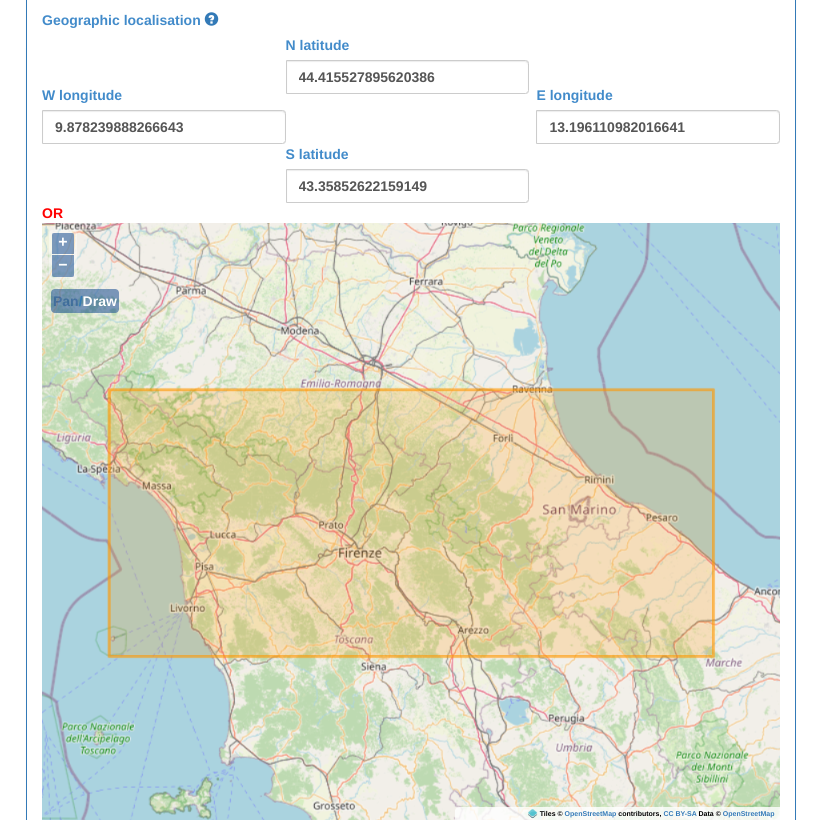
\includegraphics[width=10cm]{BoundingBox.png}
	\centering
\end{figure}	
